The following sections describe the development results of TABuss. 
\subsection{Performance}
Raaum's application suffered from poor performance. Queries took up to 40 seconds to complete, which is more than the average user is willing to wait. With the use of MultiBRIS' \cite{multibris} server, queries rarely use more than 10-15 seconds to return. 


\subsection{Optimisation with MultiBRIS' Server}

An important aspect when developing an application that uses 3G is to monitor data traffic. Table \ref{tab:without} and \ref{tab:with} display average results based on three different tests performed with the application 3G Watchdog\footnote{https://market.android.com/details?id=net.rgruet.android.g3watchdog}. The tested queries used \emph{Gl\o shaugen} as the departure stop. The first destination was set to \emph{Ila}, the second to \emph{sentrum} and the third monitored data traffic when only real-time data was downloaded.

The results especially differ in the sending of data for the queries to \emph{Ila} and \emph{Sentrum}. As MultiBRIS' server handles all computations, only one request is sent from the application to the server for each query.

Received data is also less, because only one result is returned. For the same queries in the stand-alone application, data was received from both BusTUC and the real-time system. There is also a significant reduction of downloaded data for the real-time query, because only a bus stop ID is sent from the application, and a JSON object is returned. 

It is difficult to replicate the exact same query scenarios when doing comparisons, but as the server handles both computational operations(queries to BusTUC, and real-time updates of departure times), and minimises overhead provided by SOAP messages, we can conclude that less data is sent and received. 

The stand-alone application in addition downloads a list mapping bus stop IDs to real-time IDs, on each start-up. This results in an average 400 kb of data, and is in MultiBRIS handled by the server.

\begin{table}[!h]
\caption{Data Usage without MultiBRIS' Server}
\label{tab:without}
\begin{center}
    \begin{tabular}{ |  l  |  l  |  l  |  l  |}
    \hline
    Query & Ila & Sentrum & Real-time\\ \hline
    Data sent & 5,5 kB & 8 kB & 4 kB\\ \hline
    Data received & 6,1 kB & 4,4 kB & 4,5 kB \\ \hline
    \end{tabular}
\end{center}
\end{table}

\begin{table}[!h]
\caption{Data Usage with MultiBRIS' Server}
\label{tab:with}
\begin{center}
    \begin{tabular}{ |  l  |  l  |  l  |  l  |}
    \hline
    Query & Ila & Sentrum & Real-time\\ \hline
    Data sent & 2 kB &  2 kB & 800 B\\ \hline
    Data  received & 3,5 kB & 1,5 kB & 3,5 kB \\ \hline
    \end{tabular}
\end{center}
\end{table}
\subsection{Screenshots}
\begin{figure}
\begin{tabular}{ccc}
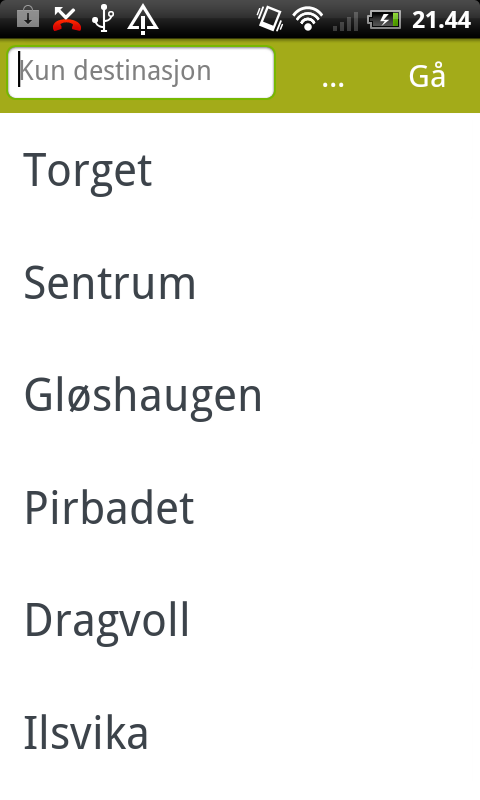
\includegraphics[width=0.27\linewidth]{Results/startscreen.png} & 
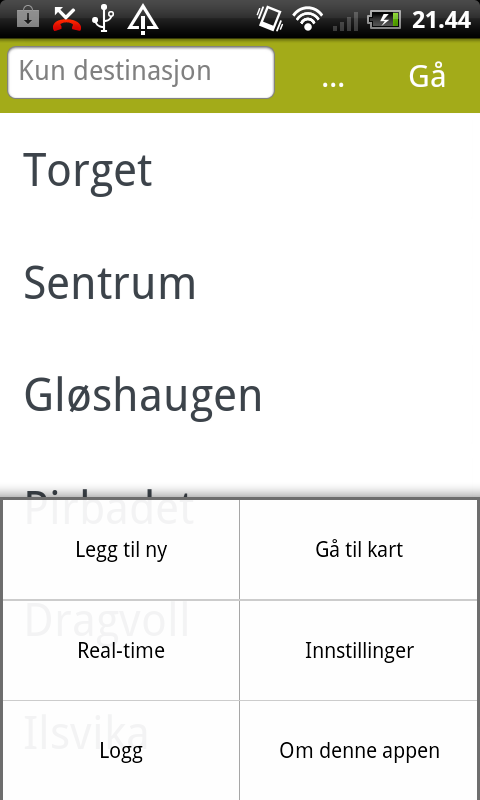
\includegraphics[width=0.27\linewidth]{Results/menu.png} &
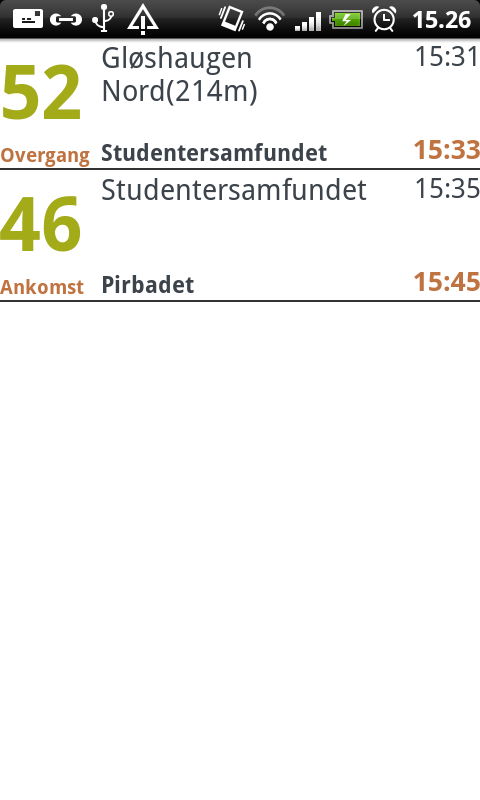
\includegraphics[width=0.27\linewidth]{Results/answer.png} \\

\includegraphics[width=0.27\linewidth]{Results/textanswer} & 
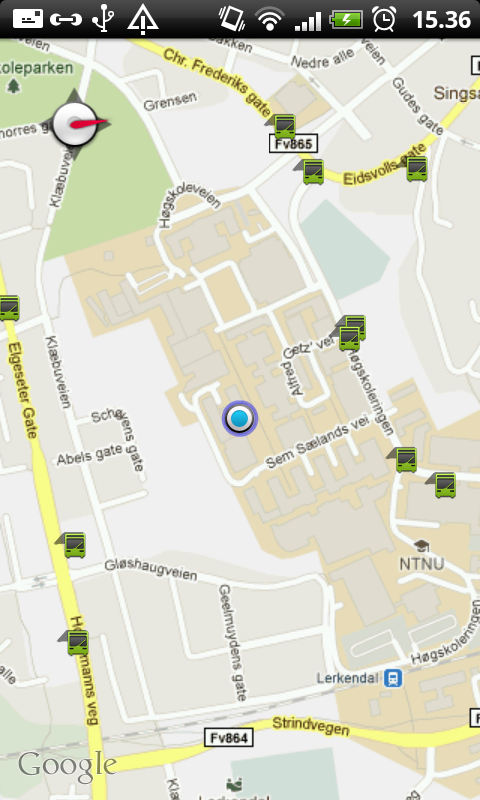
\includegraphics[width=0.27\linewidth]{Results/maprealtime.png} &
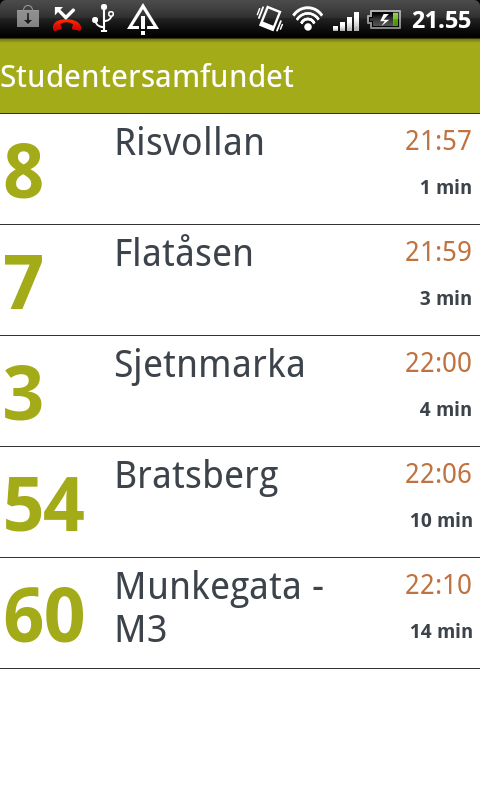
\includegraphics[width=0.27\linewidth]{Results/realtime.png} \\
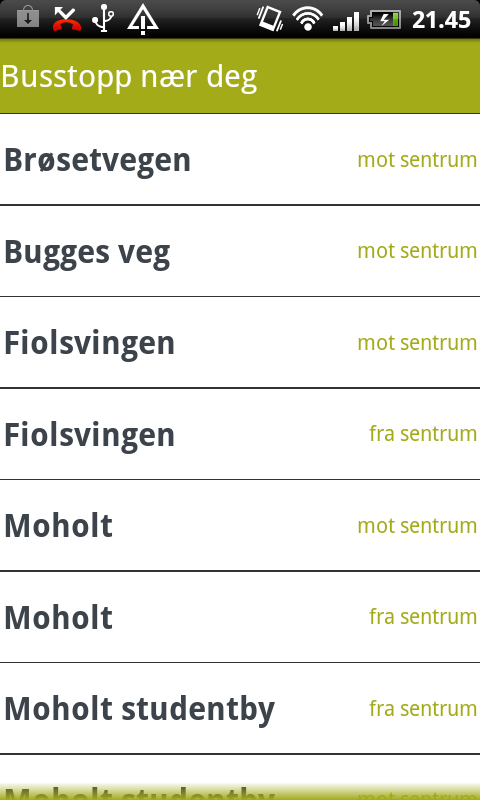
\includegraphics[width=0.27\linewidth]{Results/realtimelist.png} & 
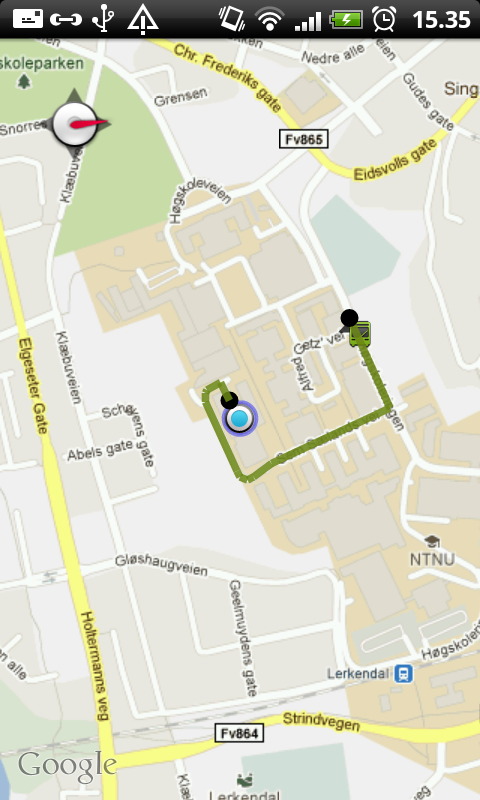
\includegraphics[width=0.27\linewidth]{Results/otherbusstop.png} &
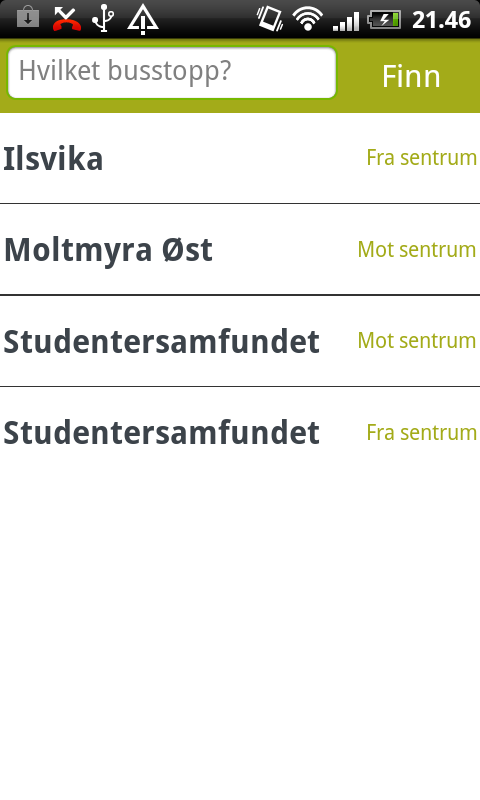
\includegraphics[width=0.27\linewidth]{Results/other.png}\\
\end{tabular}
\caption{From top left: (1)start screen, (2)menu, (3)answer screen, (4)text answer, (5)map for real-time. Displaying user location and closest bus stops, (6)real-time for stop,(7)list of real-time stops, (8)Walking route, (9)Bus stop search}
\end{figure}




\subsubsection{Screenshot Descriptions}
\begin{enumerate}
\item{Start menu where text buttons represent shortcuts stored on the device's SD-card.}
\item{Application menu. Menu elements are translated to English below. \\
\begin{table}
\caption{Translation of menu elements}
    \begin{tabular}{ |  l  |  l  |}
    \hline
    \textbf{Norwegian} & \textbf{English} \\ \hline
 Legg til ny & Add a new bus stop shortcut to the home screen\\ \hline
   Logg & Logged queries\\ \hline
    G\aa\ til kart & Proceed to map\\ \hline
   Innstillinger & Settings\\ \hline
   Om denne appen & About this application\\ \hline
    \end{tabular}
\end{table}
}
\item{The answer screen with results from a HTTP query with the new syntax. The displayed routes are the results of a BusTUC query with real-time updated departure times. In parenthesis, walking distance to the bus stop is shown. ''Overgang'' indicates the resulting route suggestions include a transfer.}
\item{The answer screen with results from a text message query with the standard syntax. Both the text message and HTTP functionality with standard syntax, will output results to this answer screen.}
\item{Map displaying user location. The closest bus stops are represented by clickable bus stop icons.}
\item{Result of a real-time data query. The query is either initiated by menu access, or by a bus stop icon press.}
\item{List of the closest bus stops to the user's location, accessed from the menu. On registered clicks, real-time data is downloaded for the selected bus stop. Each element also displays route direction, either towards or away from the city centre.}
\item{Map displaying walking route to a departure bus stop suggested by query results.}
\item{Search functionality for bus stops not in range of the user's location. If the search returns a bus stop, real-time data can be viewed. The list of elements below the input field contains recently searched bus stops. These are stored in a SQLite database.}
\end{enumerate}



\begin{figure}[!h]
\begin{tabular}{ccc}
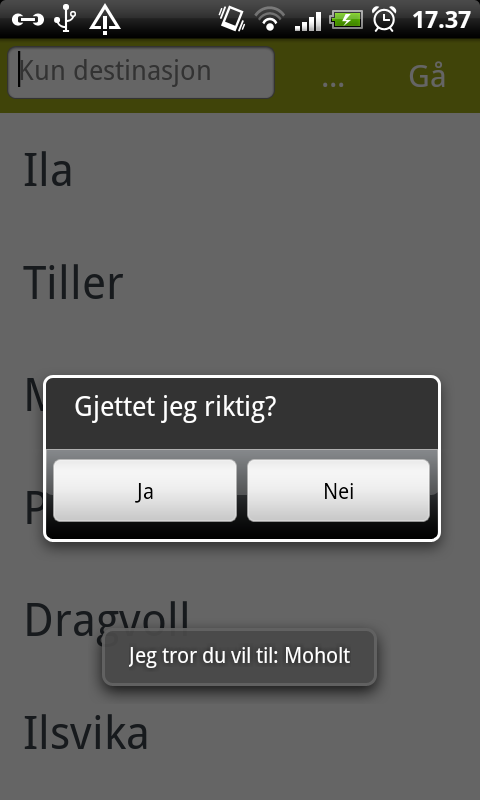
\includegraphics[width=0.27\linewidth]{Results/contextaware.png} & 
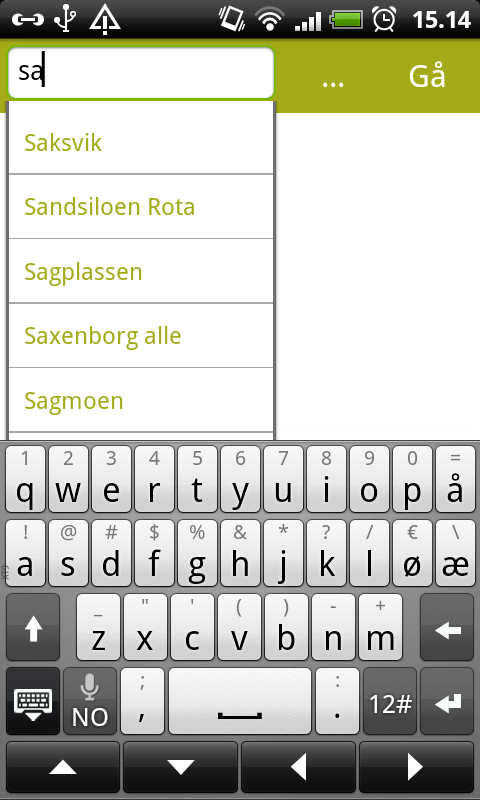
\includegraphics[width=0.27\linewidth]{Results/autocomplete.png} &
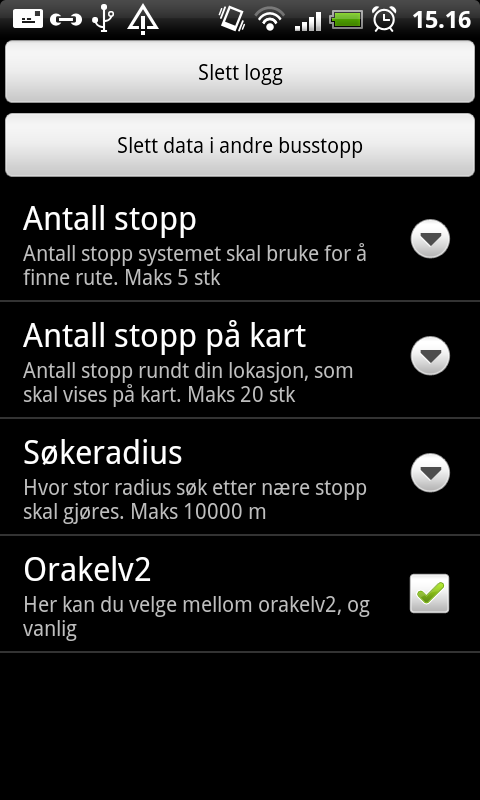
\includegraphics[width=0.27\linewidth]{Results/settings.png}\\
\end{tabular}
\caption{From left to right: (1)guess based on context, (2)autocomplete, (3)settings}
\end{figure}
\begin{enumerate}
\item{Suggestion from TABuss, based on stored cases. The bottom pop-up suggests a route, while the above dialog prompts for validation.}
\item{Autocomplete suggestions, retrieved based on the two letters entered in the input field. If clicking a suggestion, a query is run with the chosen suggestion as the departure stop.}
\item{The settings screen, where options are: delete logs, adjust number of bus stops to be included in queries with the new syntax, adjust number of bus stops to be displayed on the map, adjust search radius for bus stops and an option to switch between new and standard BusTUC syntaxes.}
\end{enumerate}
\subsection{System Testing}
TABuss has been tested before, during and after development. Most errors affecting core functionality were fixed during the testing of Raaum's application. Other errors were detected during runs, by running queries with different inputs, and also by adjusting the settings parameters. Testing was mainly done with the ''Eclipse Debugger\footnote{http://www.eclipse.org/}'', which displays error traces if exceptions occur. Our goal regarding error rate was not to achieve zero percent. With the project's time limitations, this would be too optimistic. Instead we decided to do testing continuously during implementation, fix what we could, and identify possible error sources for future reviewing. An example of a performed test was during the implementation of the error messages a user can be presented. Different scenarios were designed for the application to throw exceptions: Unmount of the SD-card after application start-up, disconnection from a network and lost location fix.

Testing without the Eclipse debugger was done by travelling routes suggested by the application. Detected exceptions were stored on the test devices' SD-cards, and reviewed when connected to a development machine.

\subsection{User Testing}
A simplified user test was performed to get feedback of TABuss' functionalities. An extensive user test was not conducted because of time limitations, and issues with permission for public release of the application. 

All of the test subjects were Trondheim inhabitants, and  experienced bus travellers.

\subsubsection{General Opinion}
The general user opinion indicated that the application was easy to use. However, some users experienced difficulties during installation, as their devices did not meet the original SDK requirements(2.3). 

It was clear that the users appreciated our prioritising of user interface. Positive feedback was received on both the colour combinations and the layout. Most users preferred the application functionalities detached from the map, and feedback suggested the map should only be an add-on.

Users found the query functionality to be useful. The main functionality with the new BusTUC syntax was seen as interesting. Accustomed to BusTUC with standard syntax, not having to provide the same amount of text was a time-saver. It was subsequently easier for the users to blame the system if an erroneous answer was returned, as user input was limited.


The real-time data functionality for the closest bus stops was a functionality found quick to access and use. This especially applied to the real-time functionality accessible from the home screen, as this required less navigation than through the map.

\subsubsection{Suggestions}
All users requested a more extensive feedback from the system, when errors occurred. Errors such as: A missing internet connection and no location fix, had up to this point been covered by a general error feedback.

For the query functionality, users requested the possibility to use the standard BusTUC syntax for queries not involving the closest located bus stops. This was not an option at the current development stage. Another suggestion was a ''settings''-screen,  allowing the user to set properties such as the number of bus stops to use in queries. 

\subsubsection{Implemented Suggestions}
When solving the installation problems some users had, a memory bug was discovered on Android 2.2. The loading and parsing of bus stop lists needed to be re-implemented, as a memory overflow occurred. The list used in Raaum's application\cite{mag} contained 498 elements, while the new lists each contains over 1000. After researching this error, a possible error source was found on a debugging forum \footnote{http://stackoverflow.com/occuring}. One forum user posted that he did not get his application to work with >505 elements. If correct, this explains why this was not detected during Raaum's project. A bug report had been filed to Google regarding this issue. The re-implementation consisted of manually parsing the XML-files,  instead of using Android's built-in parser. 

For the system feedback request, additional error messages were added. This included checks for internet connection, mounted SD-card and location fix. The usage of the standard BusTUC syntax was also implemented. The last added suggestion was a settings functionality, which lets the user set different properties within given boundaries.

\subsubsection{Conclusion}
The user's opinions were divided in the choice between the BusTUC query functionality and only real-time functionality. A possible reason may be speed, as the BusTUC query functionality during user testing was not optimised. Another reason may be the limitations some users experienced with the new BusTUC syntax. 

It is difficult to draw a concise conclusion after a narrow user test, but the feedback we received from the target users was valuable. We received implementation suggestions, information on errors and an indication that TABuss suited the needs of bus travellers. 









